\documentclass[aspectratio=169,11pt]{beamer}
\usepackage{teaching_slides}

\title[L9b - Event Studies]{ Econometrics I}
\subtitle{Lecture 8b: Event Studies}
\author{Chris Conlon \\NYU Stern}
\date{Fall 2026}

% New deck (Fall 2026). The panel event-study half takes its organizing questions
% from Paul Goldsmith-Pinkham's Applied Empirical Methods lecture 14 (Yale), used
% with attribution; the treatment here is single-timing and simulation-first, and
% leaves staggered adoption to Week 9. The CAR half follows MacKinlay (1997).
% Readings: Mixtape Ch. 9 (sections on event studies); Roth (2022, AER: Insights);
% MacKinlay (1997, JEL). Figures/tables: panel_sims.R. Workbook: inclass_session8.Rmd

\begin{document}
\maketitle

\begin{frame}{Two things called ``event study''}
\begin{itemize}
	\item \alert{The panel event study} (economics, marketing, strategy): some units experience an
	event --- a policy, a product launch, an acquisition --- at a known date. Trace the outcome
	\emph{before and after}, relative to units that did not.
	\medskip
	\item \alert{The returns event study} (finance, accounting): a firm announces something. Measure
	the stock's \emph{abnormal} return around the announcement, relative to what the market model
	predicts.
	\medskip
	\item Same skeleton in both: re-index time so the event is at zero, build a counterfactual path
	from the pre-period, and read off the gap. What differs is where the counterfactual comes from.
	\medskip
	\item Plan: the panel version (with a preview of Week 9's trouble), then the returns version.
	\medskip
	\item {\small Attribution: the questions that organize the first half --- who is the control,
	what is normalized, what does a flat pre-period buy you --- follow Goldsmith-Pinkham's
	Applied Methods lecture 14. The examples and the single-timing focus are ours.}
\end{itemize}
\end{frame}


\section{Panel event studies}

\begin{frame}{Setup: event time}
\begin{itemize}
	\item Units $i$, calendar periods $t$. Treated units all experience the event at the same
	date $E$; the rest never do. (Staggered dates: next week.)
	\medskip
	\item \alert{Event time} $k = t - E$. The period just before the event is $k = -1$.
	\medskip
	\item Potential outcomes $Y_{it}(0)$, $Y_{it}(1)$. The object we want is a whole \emph{path}:
	\begin{align*}
		\tau_k = \E\big[\,Y_{it}(1) - Y_{it}(0) \mid t - E = k,\ D_i = 1\,\big], \qquad k = 0, 1, 2, \dots
	\end{align*}
	the dynamic average treatment effect on the treated, $k$ periods after the event.
	\medskip
	\item Why a path rather than a number? Effects ramp up (adoption takes time), fade (novelty),
	or reverse (intertemporal substitution). One coefficient hides all of that, and averages it
	with weights you did not choose.
\end{itemize}
\end{frame}


\begin{frame}{The regression}
\begin{align*}
	y_{it} = \alpha_i + \gamma_t + \sum_{k \ne -1} \tau_k \cdot \mathbb{1}\{t - E = k\}\cdot D_i + \varepsilon_{it}
\end{align*}
\begin{itemize}
	\item Two-way fixed effects (last hour) plus one dummy per event time, switched on only for
	treated units.
	\medskip
	\item \alert{Reference period $k = -1$ is omitted.} Every $\tau_k$ is measured relative to the
	period before the event; $\hat\tau_{-1} \equiv 0$ by construction.
	\medskip
	\item Never-treated units have no event-time dummies. They pin down $\gamma_t$: what would have
	happened to everyone absent the event.
	\medskip
	\item Pre-period coefficients ($k < -1$) are the \emph{diagnostic}: if the treated group was
	already diverging, they will show it. Cluster by unit.
\end{itemize}
\end{frame}


\begin{frame}{Running example: an algorithmic-pricing tool}
\begin{itemize}
	\item $400$ firms observed for $24$ quarters. In quarter $13$, half of them switch on a
	pricing-optimization tool. The outcome is log gross margin.
	\medskip
	\item Ground truth: the effect ramps from $0.0125$ in the adoption quarter to $0.05$ after three
	quarters and stays there. Nothing happens before adoption.
	\medskip
	\item Also in the data: firm effects $\alpha_i$, a common macro path $\gamma_t$ (random walk with
	drift), and noise. Treated firms are not a random half --- but they are, in this first
	version, on the same trend as the others.
	\medskip
	\item Estimate the event-study regression with \texttt{fixest}'s \texttt{i()}, cluster by firm,
	and plot.
\end{itemize}
\end{frame}


\begin{frame}{The event-study plot}
\begin{center}
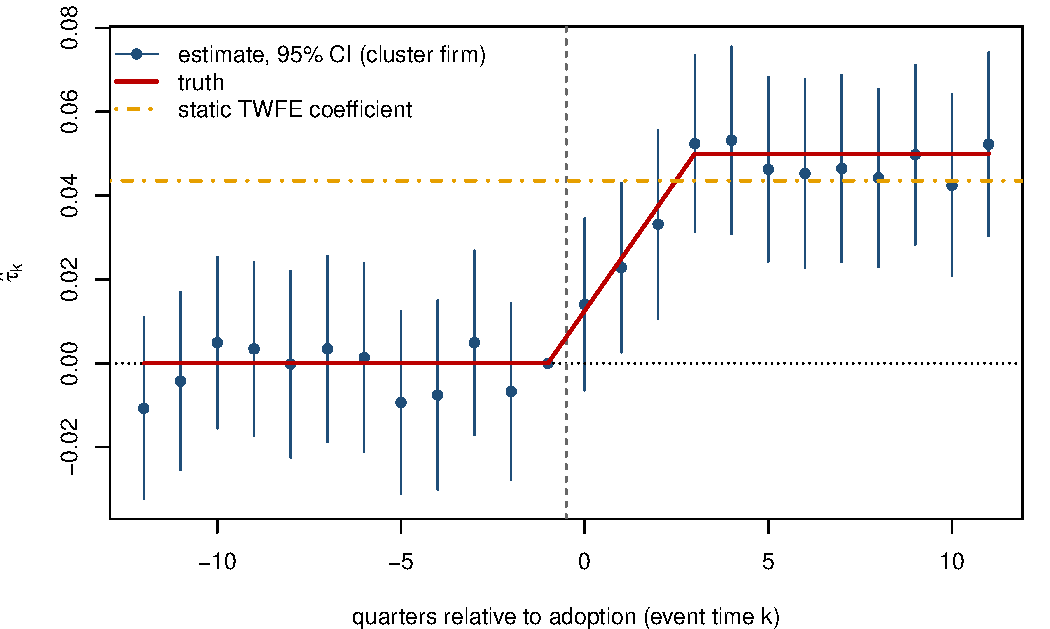
\includegraphics[width=.6\textwidth]{fig_es_single.pdf}
\end{center}
\vspace{-.3cm}
{\small Flat and near zero before, ramping after, sitting on the truth. The dashed orange line is the
\emph{single} post-period coefficient from a two-way FE regression with one treatment dummy.}
\end{frame}


\begin{frame}{How to read it}
\begin{itemize}
	\item The dot at $k = -1$ is zero \emph{by construction}. Do not read it as evidence.
	\medskip
	\item The pre-period dots test ``were the treated already moving relative to controls?'' Here
	they are not, and the confidence intervals say how big a divergence we could have seen.
	\medskip
	\item The post-period dots are $\hat\tau_k$: the effect $k$ quarters after adoption, relative to
	$k = -1$.
	\medskip
	\item The static two-way FE coefficient is a weighted average of the $\hat\tau_k$, $k \ge 0$,
	with weights proportional to how many observations sit at each $k$. With a ramp, it understates
	the long-run effect. With effects that fade, it overstates it. It is never the number you
	would have asked for.
	\medskip
	\item Confidence bands are pointwise. Twelve pre-period coefficients at $95\%$ each is not a
	$95\%$ test of ``all flat.'' Use a joint (Wald) test, or a uniform band.
\end{itemize}
\end{frame}


\begin{frame}{Assumptions, stated properly}
\begin{enumerate}
	\item \alert{Parallel trends} in event time: absent the event, treated and control paths would
	have moved together,
	\begin{align*}
		\E[Y_{it}(0) - Y_{is}(0) \mid D_i = 1] = \E[Y_{it}(0) - Y_{is}(0) \mid D_i = 0] \quad \forall\, t, s .
	\end{align*}
	\medskip
	\item \alert{No anticipation}: $Y_{it}(1) = Y_{it}(0)$ for $t < E$. Units do not act on the
	event before it happens.
\end{enumerate}
\medskip
\begin{itemize}
	\item Under both, $\hat\tau_k$ is consistent for the dynamic ATT and $\tau_k = 0$ for $k < 0$.
	\medskip
	\item Only the \emph{implication} ($\hat\tau_k \approx 0$ for $k < -1$) is testable. Parallel
	trends in the post-period is an assumption about a counterfactual you never see.
	\medskip
	\item Both are assumptions about \emph{levels of $Y(0)$ differences}, not about levels of $Y$.
	Treated firms can be bigger, older, richer. They cannot be on a different trajectory.
\end{itemize}
\end{frame}


\begin{frame}{What a flat pre-period does not buy you}
\begin{center}
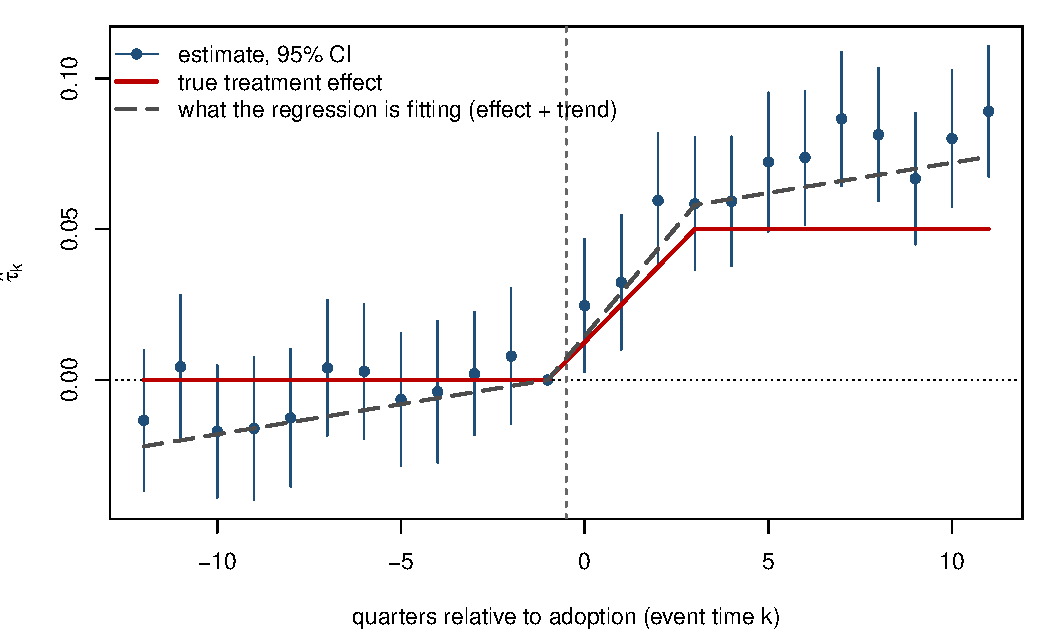
\includegraphics[width=.58\textwidth]{fig_es_pretrend.pdf}
\end{center}
\vspace{-.3cm}
{\small Same design, plus a differential trend of $0.2\%$ per quarter for treated firms. No
pre-period dot is individually significant and the joint test does not reject ($p = 0.30$). The
post-period estimates are biased upward, and the bias grows with $k$.}
\end{frame}


\begin{frame}{The pre-test problem (Roth 2022)}
\begin{itemize}
	\item A pre-trend test has power only against violations large relative to the noise. When the
	violation is small, the test passes and the bias is still there.
	\item Worse: \alert{conditioning on passing} selects samples where pre-period noise offset the
	trend; the post-period estimates in those samples are biased \emph{more}, not less.
	\item A linear trend with slope $\delta$ biases $\hat\tau_k$ by $\delta\,(k + 1)$: the further
	out you look, the worse it gets, while the pre-test's power is fixed.
\end{itemize}
\vspace{-.2cm}
\begin{center}
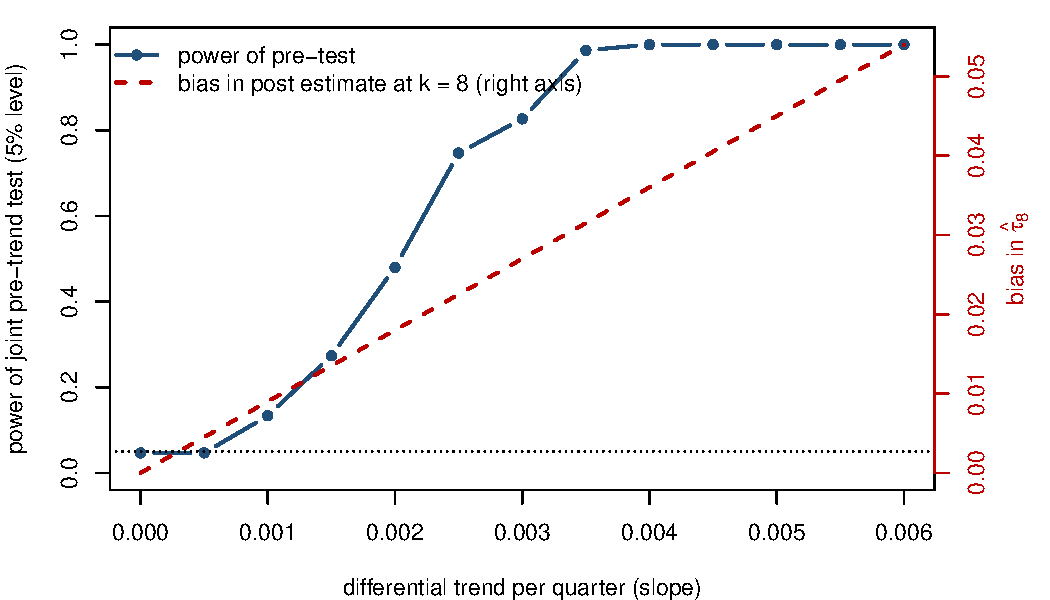
\includegraphics[width=.38\textwidth]{fig_es_pretest_power.pdf}
\end{center}
\end{frame}


\begin{frame}{What to do instead}
\begin{itemize}
	\item \alert{Plot, and report magnitudes.} ``The pre-period coefficients are individually
	insignificant'' is not a finding. ``The data rule out a pre-trend larger than $x$ per quarter,
	which would bias $\hat\tau_8$ by at most $9x$'' is.
	\medskip
	\item \alert{Sensitivity analysis.} Rambachan and Roth (2023): allow the post-period violation
	to be as large as (some multiple of) the largest pre-period violation, and report the range of
	$\tau_k$ consistent with that. \texttt{HonestDiD} does it in a few lines.
	\medskip
	\item \alert{Longer pre-periods} help detect trends; they do not help if the trend is real.
	\medskip
	\item \alert{Detrend only with care.} Fitting a treated-group trend on the pre-period and
	extrapolating it assumes the trend would have continued --- a strong claim about a
	counterfactual, and it eats precision.
	\medskip
	\item \alert{A better control group} is worth more than any of the above. Firms in the same
	segment, matched on pre-period trajectory, or --- next week --- a synthetic control.
\end{itemize}
\end{frame}


\begin{frame}{Anticipation}
\begin{center}
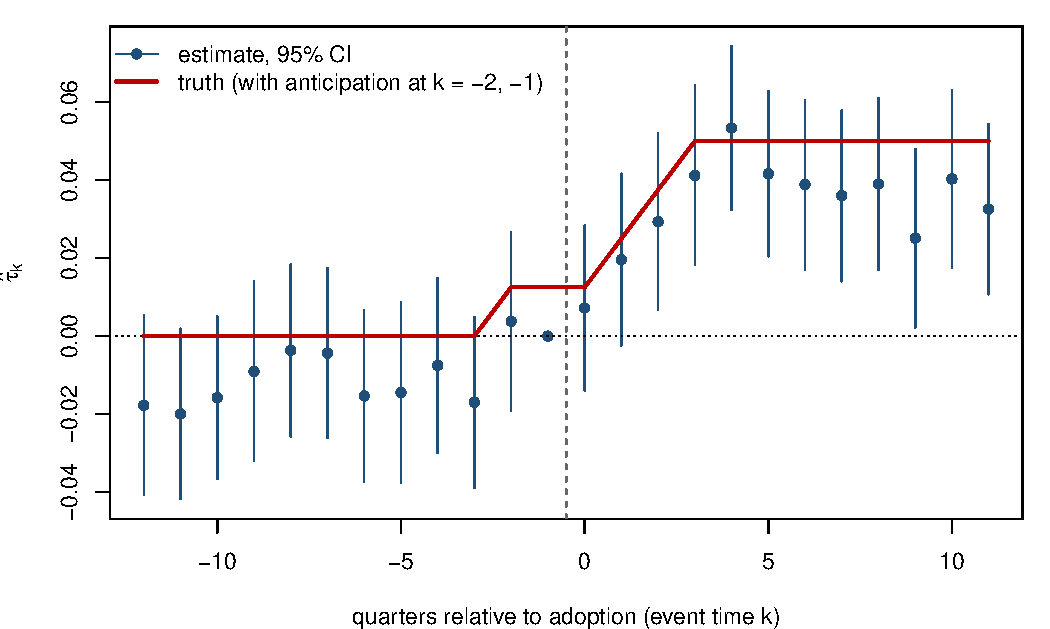
\includegraphics[width=.55\textwidth]{fig_es_anticipation.pdf}
\end{center}
\vspace{-.3cm}
{\small Firms start adjusting two quarters before the tool goes live (pilot programs, contract
renegotiation). The pre-period now shows a bump; and since $k = -1$ is the reference, every
\emph{post}-period estimate is shifted down by the anticipation effect. Fix: set the reference to
$k = -3$, or redefine the event date as the announcement.}
\end{frame}


\begin{frame}{Design choices you will have to make}
\begin{itemize}
	\item \alert{Who is the control?} Never-treated units are cleanest. If everyone is treated
	eventually, not-yet-treated units serve until their own event (staggered: next week).
	\item \alert{No control group at all?} With a single event date and everyone treated, event
	time \emph{is} calendar time. The event-time dummies are collinear with $\gamma_t$. \texttt{fixest} says
	``without doubt, your model is misspecified,'' and it is right: you would be assuming the
	counterfactual is flat.
	\item \alert{Window and binning.} Estimate $\tau_k$ for $k \in [-K_0, K_1]$ and bin everything
	outside into endpoint dummies, so far-out observations do not form a category of three firms.
	\item \alert{Balance in event time.} If the panel is unbalanced, $\hat\tau_6$ comes from
	different firms than $\hat\tau_2$, and composition changes look like dynamics. Restrict to firms
	observed over the whole window, or say why not.
	\item \alert{Reference period.} $k = -1$ by convention; earlier if anticipation is plausible.
\end{itemize}
\end{frame}


\begin{frame}{Where it comes from: difference-in-differences in disguise}
\begin{itemize}
	\item Take two periods, $t \in \{E-1, E+k\}$, and the two groups. The event-study coefficient is
	\begin{align*}
		\hat\tau_k = \big(\bar y^{\,T}_{E+k} - \bar y^{\,T}_{E-1}\big) - \big(\bar y^{\,C}_{E+k} - \bar y^{\,C}_{E-1}\big),
	\end{align*}
	a $2 \times 2$ difference-in-differences comparing period $k$ to the reference period.
	\medskip
	\item So the event study is a \emph{collection} of DiD estimates, one per $k$, sharing a
	baseline. Everything you learn about DiD next week applies coefficient by coefficient.
	\medskip
	\item Equivalently: the regression is fitting each period's treated-minus-control gap and
	subtracting the gap at $k = -1$.
\end{itemize}
\end{frame}


\begin{frame}[fragile]{In practice}
\begin{lstlisting}
es[, k := ifelse(treated == 1, t - 13, -1)]              # controls get the reference value
fit <- feols(y ~ i(k, ref = -1) | firm + t, es, cluster = ~firm)
iplot(fit, ref.line = -0.5)                                # the event-study plot
wald(fit, keep = "k::-")                                   # joint test on pre-period coefficients
\end{lstlisting}
\begin{lstlisting}[language=Python]
es["k"] = np.where(es.treated == 1, es.t - 13, -1)
fit = pf.feols("y ~ i(k, ref=-1) | firm + t", data=es, vcov={"CRV1": "firm"})
fit.iplot()
\end{lstlisting}
\begin{itemize}
	\item Binning: recode $k$ to $\min(\max(k, -K_0), K_1)$ before \texttt{i()}.
	\item Never-treated units should carry the reference value, not \texttt{NA}: they must stay in the
	regression to estimate $\gamma_t$.
\end{itemize}
\end{frame}


\begin{frame}{Preview of Week 9: staggered adoption breaks this}
\begin{itemize}
	\item Today every treated firm adopted in quarter 13. In practice adoption is
	\alert{staggered}: cohorts $g = 2019, 2020, 2021, \dots$
	\medskip
	\item The same two-way FE regression then uses \emph{already-treated} firms as controls for
	later cohorts. If effects are dynamic, those ``controls'' are moving, and the comparison is
	contaminated (Goodman-Bacon 2021; Sun and Abraham 2021).
	\medskip
	\item Symptoms: negative weights on some cohorts; pre-period coefficients that are non-zero
	even when there is no pre-trend; post-period coefficients that mix cohorts' dynamics.
	\medskip
	\item Fixes (next week): estimate cohort-by-event-time effects and aggregate them yourself
	(Callaway--Sant'Anna, Sun--Abraham, Borusyak--Jaravel--Spiess imputation).
	\medskip
	\item The single-timing case is the one where two-way FE is exactly right. Know what
	``right'' looks like before we break it.
\end{itemize}
\end{frame}


\section{Returns event studies}

\begin{frame}{The returns event study}
\begin{itemize}
	\item Ball and Brown (1968), Fama, Fisher, Jensen and Roll (1969): does the stock market react to
	news, and how fast? Still the workhorse of empirical accounting and corporate finance.
	\medskip
	\item Typical events: earnings announcements, M\&A announcements, CEO turnover, index inclusion,
	regulatory actions, product recalls, data breaches.
	\medskip
	\item The logic is the panel event study with one change: the counterfactual for firm $i$
	is not other firms, it is \alert{firm $i$'s own relationship to the market}, estimated on
	pre-event data.
	\medskip
	\item The panel is long and narrow per event ($T \approx 250$ trading days per firm) rather than
	short and wide. So the ``fixed effect'' is estimated well, and the interesting inference is
	cross-sectional: averaging across events.
	\medskip
	\item Reference: MacKinlay (1997, \emph{JEL}), ``Event Studies in Economics and Finance.''
\end{itemize}
\end{frame}


\begin{frame}{Setup}
\begin{itemize}
	\item Event day $0$ for firm $i$. \alert{Estimation window} $[-250, -11]$; \alert{event window}
	$[-10, +10]$. The gap keeps the event out of the estimation sample.
	\medskip
	\item \alert{Market model}, estimated on the estimation window by OLS, one firm at a time:
	\begin{align*}
		R_{it} = a_i + b_i R_{mt} + e_{it}, \qquad \E[e_{it} \mid R_{mt}] = 0 .
	\end{align*}
	\medskip
	\item \alert{Abnormal return} on the event window: actual minus predicted,
	\begin{align*}
		\widehat{AR}_{it} = R_{it} - \hat a_i - \hat b_i R_{mt} .
	\end{align*}
	\medskip
	\item \alert{Cumulative abnormal return} over a window $[k_1, k_2]$:
	$\widehat{CAR}_i(k_1, k_2) = \sum_{t = k_1}^{k_2} \widehat{AR}_{it}$.
	\item Compare to the panel version: $a_i$ is $\alpha_i$, $b_i R_{mt}$ is $\gamma_t$ with a
	firm-specific loading, and $AR_{it}$ is $\hat\tau_k$ for one firm.
\end{itemize}
\end{frame}


\begin{frame}{Simulated example: earnings announcements}
\begin{itemize}
	\item $200$ firms, each with one announcement. Daily returns for $261$ days per firm.
	\medskip
	\item Market return $R_{mt} \sim N(0.04\%,\ 1\%^2)$, common to all firms on a given day.
	Betas $b_i \sim N(1, 0.3^2)$; idiosyncratic volatility $2\%$ per day.
	\medskip
	\item Each firm has a standardized \alert{earnings surprise} $S_i \sim N(0, 1)$.
	Ground truth for the abnormal return:
	\begin{align*}
		AR_{i0} = 0.02\, S_i, \qquad AR_{it} = 0.001\, S_i \ \text{ for } t = 1, \dots, 10, \qquad 0 \text{ otherwise}.
	\end{align*}
	A one-SD surprise moves the stock $2\%$ on the day and drifts another $1\%$ over two weeks
	(post-earnings-announcement drift, Bernard and Thomas 1989).
	\medskip
	\item So $CAR_i(0, 10) = 0.03\, S_i$ in expectation, and $CAR_i(-10, -2) = 0$.
\end{itemize}
\end{frame}


\begin{frame}{One firm}
\begin{center}
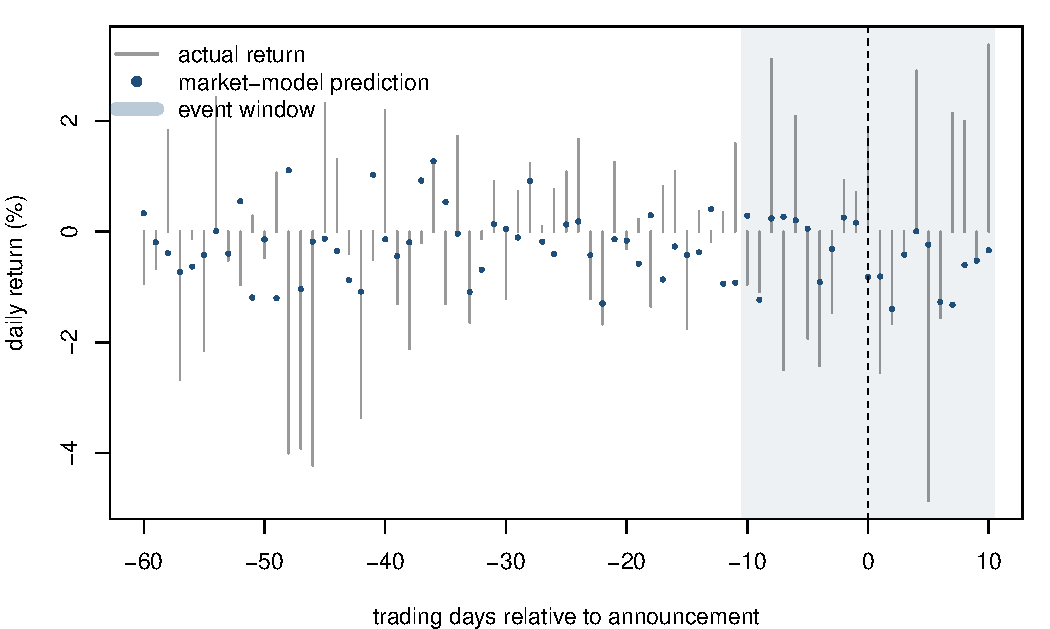
\includegraphics[width=.55\textwidth]{fig_car_onefirm.pdf}
\end{center}
\vspace{-.3cm}
{\small The firm with the largest positive surprise. Grey bars are actual daily returns; blue dots the
market-model prediction. The abnormal return is the gap, and on day $0$ it is hard to miss. On most
other days it is noise of $\pm 2\%$: one firm tells you little.}
\end{frame}


\begin{frame}{Averaging across firms}
\begin{center}
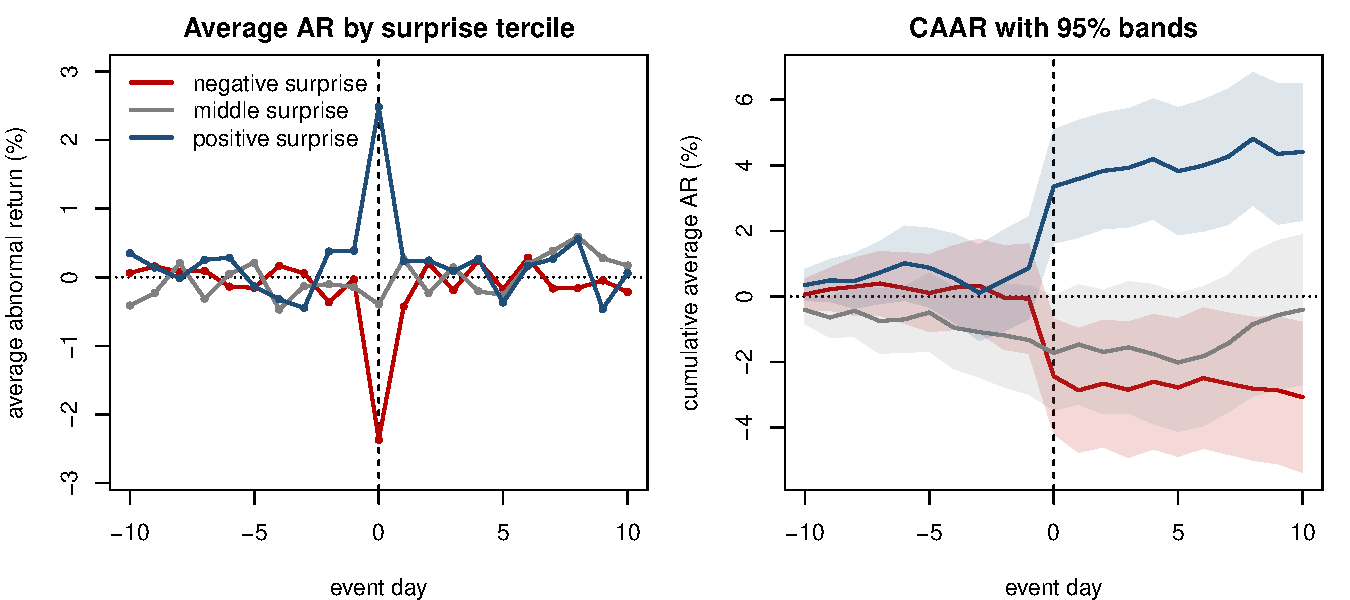
\includegraphics[width=.78\textwidth]{fig_car_aar.pdf}
\end{center}
\vspace{-.2cm}
{\small Left: the average abnormal return by event day, by tercile of surprise. Right: cumulated. The
day-$0$ jump and the post-announcement drift are both visible once you average over $\approx 67$ firms.
Nothing happens before day $0$: the analog of a flat pre-period.}
\end{frame}


\begin{frame}{Inference}
\begin{itemize}
	\item Under the null of no abnormal return, $\widehat{AR}_{it}$ has mean zero and variance
	$\sigma^2_{e,i}\,(1 + \text{small estimation-error term})$; over a window of length $L$,
	$\Var[\widehat{CAR}_i] \approx L\,\sigma^2_{e,i}$.
	\medskip
	\item Two standard test statistics for the \alert{average} CAR across $N$ events:
	\begin{itemize}
		\item \alert{Cross-sectional $t$}: treat the $N$ CARs as an i.i.d.\ sample. Robust to
		event-induced variance changes; needs $N$ moderately large.
		\item \alert{Standardized} (Patell 1976; Boehmer et al.\ 1991): scale each firm's CAR by its own
		$\hat\sigma_{e,i}\sqrt{L}$ first, then average. Better power when volatility differs across firms.
	\end{itemize}
	\medskip
	\item Both assume independence \emph{across firms}. That fails when events cluster in calendar
	time (every firm announces in the same week; a regulation hits every bank on the same day).
	Then the market-model residuals are cross-sectionally correlated and the $t$-statistics are too
	large --- the same clustering problem as Week 3, in a different costume. Fix: calendar-time
	portfolios, or cluster by event date.
\end{itemize}
\end{frame}


\begin{frame}{CARs by window}
\begin{center}
\begin{tabular}{lccccc}\toprule
Window & CAAR (\%) & $t$ (cross-section) & $t$ (standardized) & CAAR, $S>0$ & CAAR, $S<0$ \\ \midrule
$[-10, -2]$ & -0.25 & -0.54 & -0.57 & 0.17 & -0.56 \\
$[-1, 1]$ & -0.02 & -0.05 & -0.08 & 2.71 & -2.03 \\
$[0, 0]$ & -0.11 & -0.53 & -0.75 & 2.06 & -1.71 \\
$[1, 10]$ & 0.58 & 1.38 & 1.30 & 1.22 & 0.10 \\
$[0, 10]$ & 0.47 & 1.01 & 1.02 & 3.28 & -1.61 \\
\bottomrule\end{tabular}

\end{center}
\medskip
\begin{itemize}
	\item The pre-event window is indistinguishable from zero; the announcement windows are not, once
	you split by the sign of the surprise. (Pooled over all firms, the average CAR is near zero because
	surprises average to zero. The \emph{sign} of $S_i$ is the treatment.)
	\item The two test statistics agree here because all firms have similar volatility.
\end{itemize}
\end{frame}


\begin{frame}{The cross-sectional regression}
The quantity accounting cares about is the \alert{earnings response coefficient}: how much return per unit of surprise.
\begin{columns}[T]
\begin{column}{0.5\textwidth}
\begin{center}
\begin{tabular}{lc}\toprule
 & $\widehat{\text{CAR}}_i(0,10)$ on $S_i$ \\ \midrule
Slope on surprise $S_i$ (truth $= 0.030$) & 0.0244 (0.0037) \\
Intercept & 0.0068 (0.0043) \\
$N$ firms, $R^2$ & 200, 0.16 \\
\bottomrule\end{tabular}

\end{center}
\medskip
{\small Regress $\widehat{CAR}_i(0, 10)$ on $S_i$ with heteroskedasticity-robust standard errors. The
slope recovers the truth. This is the CAR analog of putting a covariate in the event-study regression.}
\end{column}
\begin{column}{0.5\textwidth}
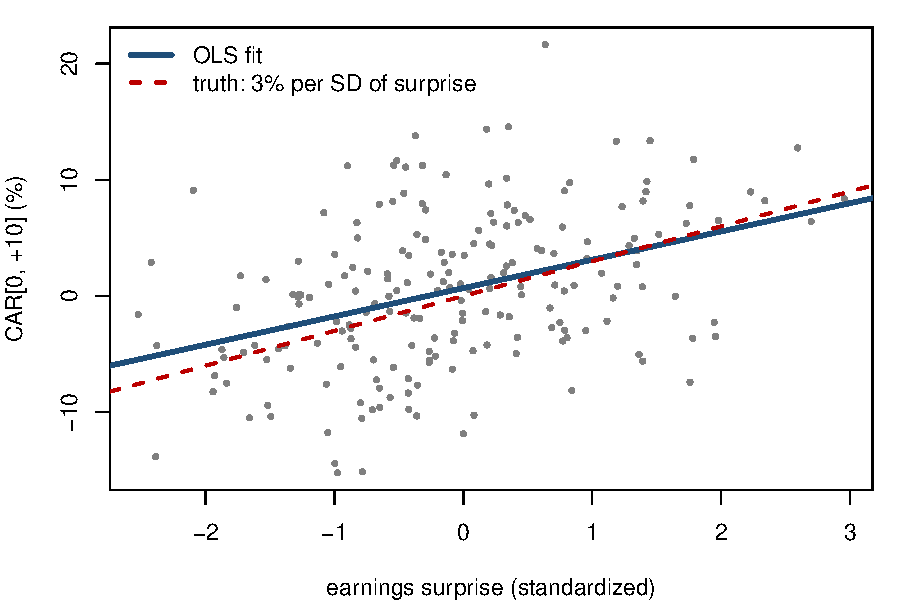
\includegraphics[width=\textwidth]{fig_car_erc.pdf}
\end{column}
\end{columns}
\end{frame}


\begin{frame}{What can go wrong}
\begin{itemize}
	\item \alert{Confounding events.} A dividend change announced with earnings; a merger rumor the
	day before. Short windows help; reading the news for each event helps more.
	\medskip
	\item \alert{Event-date uncertainty.} Information leaks; after-hours announcements land on the
	next trading day. Widen the window, at the cost of noise.
	\medskip
	\item \alert{The joint-hypothesis problem.} ``Abnormal'' is relative to a model. If the market
	model is wrong (missing factors, time-varying beta), so is the abnormal return. Over days it barely
	matters; over months or years (long-horizon ``BHAR'' studies) it dominates.
	\medskip
	\item \alert{Thin trading and non-synchronous prices} bias $\hat b_i$ for small stocks.
	\medskip
	\item \alert{Selection into the event.} Firms choose when to announce, whether to do a buyback,
	whether to be acquired. The CAR measures the market's reaction \emph{conditional on the firm
	having chosen the event}. That is often what you want; it is not the effect of assigning the
	event at random.
\end{itemize}
\end{frame}


\begin{frame}{Recap}
\begin{itemize}
	\item An event study re-indexes time to the event and compares the outcome path to a
	counterfactual path.
	\medskip
	\item \alert{Panel version}: two-way FE plus event-time dummies, reference $k = -1$, never-treated
	controls estimate $\gamma_t$. Needs parallel trends and no anticipation. The pre-period is a
	diagnostic with limited power; report what it rules out, not just whether it passed.
	\medskip
	\item \alert{Returns version}: the market model is the counterfactual, estimated per firm on the
	pre-window. Abnormal returns, cumulated and averaged; cross-sectional $t$ or standardized tests;
	watch for clustered event dates.
	\medskip
	\item Both are collections of difference-in-differences. Next week: what happens when the
	events happen at different times.
\end{itemize}
\end{frame}


\begin{frame}{Workbook time}
\texttt{inclass\_session8.Rmd}, second half:
\begin{enumerate}
	\item Reproduce the event-study plot and the joint pre-trend test. Then add anticipation and fix
	it by changing the reference period.
	\item Reproduce the CAR table. Then move every firm's announcement to the same calendar day and
	add a common market shock on that day. What happens to the $t$-statistics, and why?
\end{enumerate}
\end{frame}

\end{document}
